\documentclass[a4paper]{article}
\usepackage{amsfonts}
\usepackage{amsmath}
\usepackage{amssymb}
\usepackage{graphicx}      

\newcommand{\dint}{\displaystyle\int}
\newcommand{\dsum}{\displaystyle\sum}
\newcommand{\Bgsin}{\operatorname{Bgsin}}
\newcommand{\Bgcos}{\operatorname{Bgcos}}
\newcommand{\Bgtan}{\operatorname{Bgtan}}

\begin{document}
  
\noindent \large Auteur: Thijs Van Schel \\
\noindent \large Studierichting: Informatica\\
\noindent \large Oefeningenreeks 3G nr. 18.5\\

\medskip

\normalsize

\begin{enumerate}
    \item Domein: $\mathbb{R}$\\

    \item Asymptoten:\\
    
    Verticale asymptoten:\\
    
    geen nulpunten in de noemer $\Rightarrow$ geen VA\\
    
    Horizontale asymptoten:\\
    
    $\lim\limits_{x \to +\infty} \sqrt[3]{x^3-3x+2} = +\infty$\\
    
    $\lim\limits_{x \to -\infty} \sqrt[3]{x^3-3x+2} = -\infty$\\
    
    geen horizontale asymptoten\\
    
    Schuine asymptoot:\\
    
    $y = \sqrt[3]{x^3-3x+2}$\\
    
    $y^3 = x^3 - 3x + 2$\\
    
    $y = ax + b \Rightarrow y^3 = (ax+b)^3$\\
    
    $y^3 = a^3x^3 + 3a^2bx^2 + 3ab^2x + b^3$\\
    
    $\left\{
        \begin{array}{l}
            a^3 = 1 \Rightarrow a = 1\\
            3a^2b = 0 \Rightarrow b = 0\\
        \end{array}
    \right.$\\
    
    $y = x$\\
    
    Ligging ten opzichte van SA:\\
    
    $(f(x))^3 - y^3 = (x^3-3x+2) - x^3 = -3x+2$\\
    
    \begin{tabular}{c|ccc}
    $x$ & & $\dfrac{2}{3}$ & \\ \hline
    $(f(x))^3-y^3$ & $+$ & $0$ & $-$ \\ \hline
    & boven & snijpunt & onder
    \end{tabular} \\

    \item Tekenonderzoek $f(x)$:\\
    
    $f(x) = 0 \Leftrightarrow x^3 - 3x + 2 = 0$\\
    
    $(x-1)^2(x+2) = 0$\\
    
    $x = 1 $ of $ x = -2$\\

    \item Tekenonderzoek $f'(x)$:\\
    
    $f'(x) = \left((x^3-3x+2)^{\tfrac{1}{3}}\right)'$\\
    
    $f'(x) = \tfrac{1}{3}(x^3-3x+2)^{-\tfrac{2}{3}}(3x^2-3)$\\
    
    $f'(x) = \dfrac{x^2-1}{(x^3-3x+2)^{\tfrac{2}{3}}}$\\
    
    $f'(x) = \dfrac{(x-1)(x+1)}{((x-1)^2(x+2))^{\tfrac{2}{3}}}$\\
    
    $f'(x) = \dfrac{x+1}{(x-1)^{\tfrac{1}{3}}(x+2)^{\tfrac{2}{3}}}$\\
    
    $f'(x) = 0 \Leftrightarrow x = -1$\\

    \item Tekenonderzoek $f''(x)$:\\
    
    $f''(x) = \left( \dfrac{x^2-1}{(x^3-3x+2)^{\tfrac{2}{3}}} \right)'$\\
    
    $f''(x) = \dfrac{2x(x^3-3x+2)^{\tfrac{2}{3}} - (x^2-1)\left(\tfrac{2}{3}(x^3-3x+2)^{-\tfrac{1}{3}}(3x^2-3)\right)}{(x^3-3x+2)^{\tfrac{4}{3}}}$\\
    
    $f''(x) = \dfrac{2x(x^3-3x+2) - 2(x^2-1)^2}{(x^3-3x+2)^{\tfrac{5}{3}}}$\\
    
    $f''(x) = \dfrac{2x^4-6x^2+4x - (2x^4-4x^2+2)}{(x^3-3x+2)^{\tfrac{5}{3}}}$\\
    
    $f''(x) = \dfrac{-2x^2+4x-2}{((x-1)^2(x+2))^{\tfrac{5}{3}}}$\\
    
    $f''(x) = \dfrac{-2(x-1)^2}{(x-1)^{\tfrac{10}{3}}(x+2)^{\tfrac{5}{3}}}$\\
    
    $f''(x) = \dfrac{-2}{(x-1)^{\tfrac{4}{3}}(x+2)^{\tfrac{5}{3}}}$\\

    \item Tekentabel:\\
    
    \begin{tabular}{c|ccccccc}
    $x$ & & $-2$ & & $-1$ & & $1$ & \\ \hline
    $f(x)$ & $-$ & $0$ & $+$ & $\sqrt[3]{4}$ & $+$ & $0$ & $+$ \\
    $f'(x)$ & $+$ & $+\infty$ & $+$ & $0$ & $-$ & $\pm\infty$ & $+$ \\
    $f''(x)$ & $+$ & $|$ & $-$ & $-$ & $-$ & $|$ & $-$ \\ \hline
    $f(x)$ & $\nearrow$ & $BP(0)$ & $\nearrow$ & $M\left(\sqrt[3]{4}\right)$ & $\searrow$ & $m(0)$ & $\nearrow$ \\
           & $\smile$ & & $\frown$ & & $\frown$ & & $\frown$
    \end{tabular} \\

\end{enumerate}

\begin{figure}[h]
    \centering
    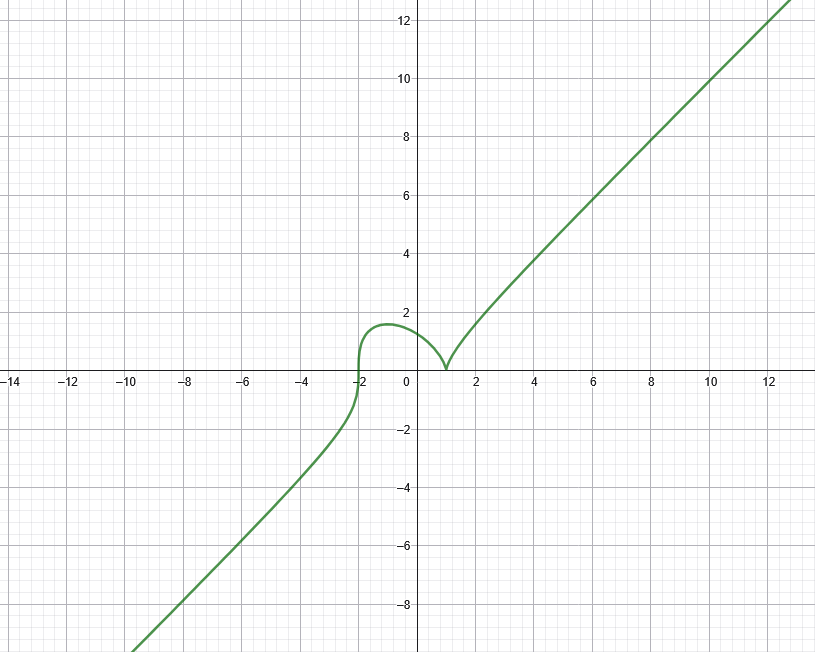
\includegraphics[width=0.6\textwidth]{3G-18.5-thijs.van.schel.INF.png}
\end{figure}

\begin{thebibliography}{999}
%\bibitem{a} Referentie
\end{thebibliography}
\end{document}